6.-
Describe un autómata que produzca el lenguaje $L = \{w \in \{a, b\}^* : |w|_a \equiv 0 \pmod 3\}$, argumenta.
\bigskip



\textbf{Definición formal del autómata:}

El Autómata se define:

\bigskip

\begin{figure}[H]
    \centering
    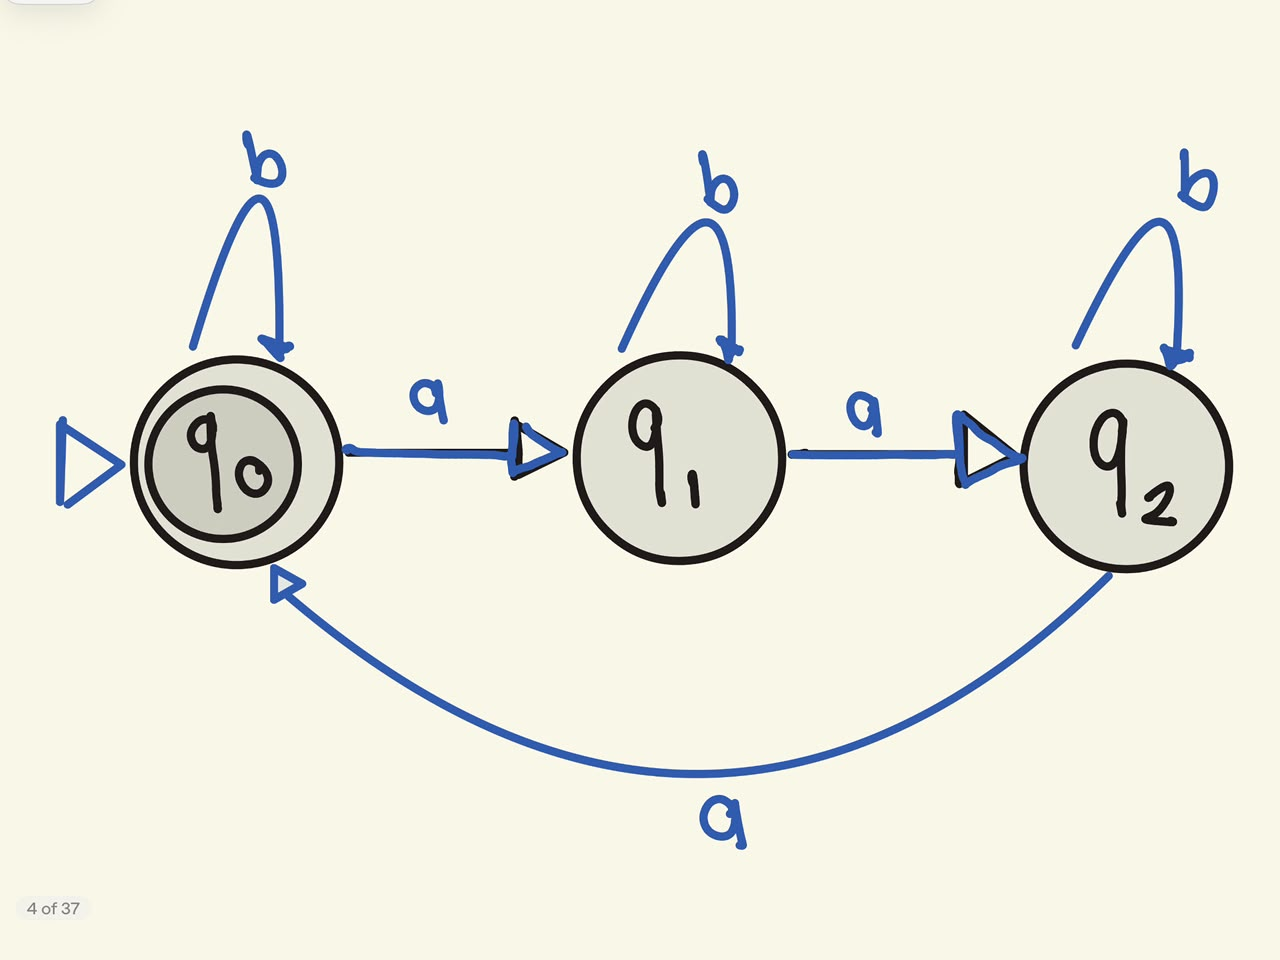
\includegraphics[width=0.5\linewidth]{recursos/aut.jpeg}
\end{figure}

\begin{itemize}
    \item \textbf{Estados ($Q$):} $\{q_0, q_1, q_2\}$
    \item \textbf{Alfabeto ($\Sigma$):} $\{a, b\}$
    \item \textbf{Estado inicial ($q_0$):} $q_0$
    \item \textbf{Estados de aceptación ($F$):} $\{q_0\}$
\end{itemize}

\textbf{Semántica de los estados:}
\begin{itemize}
    \item $q_0$: El número de letras $a$ procesadas es múltiplo de 3 (residuo 0).
    \item $q_1$: El número de letras $a$ procesadas deja un residuo de 1 al dividir entre 3.
    \item $q_2$: El número de letras $a$ procesadas deja un residuo de 2 al dividir entre 3.
\end{itemize}

\bigskip

\textbf{Argumento de correctitud:}
\bigskip

El autómata funciona como un contador circular de tres posiciones ($q_0$, $q_1$, $q_2$) que registra el residuo de dividir la cantidad de letras $a$ entre tres, ignorando por completo las letras $b$ mediante bucles que lo mantienen en su estado actual. Al iniciar en $q_0$ (residuo cero), cada nueva $a$ lo hace avanzar un paso, de modo que la primera lo lleva a $q_1$ (sobra una), la segunda a $q_2$ (sobran dos), y la tercera cierra el ciclo regresándolo a $q_0$; debido a que $q_0$ es su único estado de aceptación, el autómata garantiza que la cadena de texto solo sea aprobada si las letras $a$ completan ciclos exactos de tres, asegurando que su cantidad sea un múltiplo de 3 sin importar cuántas $b$ existan en la palabra.
